\section{Ma mission}

% L'étudiant décrit les missions menées pendant le stage. Ces missions peuvent être présentées sous une logique chronologique ou thématique. L'étudiant optera pour une logique thématique si le stage était basé sur des activités récurrentes. Et optera pour une logique chronologique si le stage était basé sur des activités très diverses. C’est ainsi qu’il pourra décrire les postes de travail occupés, expliquer ses tâches et faire part des contacts avec les différents acteurs de l'entreprise (services ou personnes).

\subsection{Mission}

Au cours de mon stage, j'ai entrepris diverses missions au sein de l'association dans le but de mener à bien le projet qui m'a été confié.

Initialement, je vais détailler en profondeur le projet qui m'a été attribué, puis je vais fournir des explications approfondies sur les différentes tâches entreprises pour la réalisation réussie de ce projet.

\subsubsection{Le projet}

Le projet consiste en la création d'une application interne à l'école CY~Tech, visant à améliorer la communication des associations étudiantes concernant les événements qu'elles organisent. Cette application offre aux étudiants la possibilité de s'inscrire aisément aux événements et de rester informés plus facilement de ce qui se passe autour d'eux.

Le projet est subdivisé en deux sous-projets : le développement d'une application web et la création d'une API.

L'application web fait office d'interface graphique entre l'utilisateur et l'API, assurant la liaison entre la base de données et l'interface utilisateur. Nous avons fait le choix de diviser le projet en deux parties distinctes pour garantir une maintenance optimale des applications et permettre à plusieurs applications web de bénéficier de ce service.

Plusieurs fonctionnalités essentielles sont prévues pour les applications :
\begin{itemize}
	\item Création et gestion de comptes utilisateurs ;
	\item Abonnement aux associations ;
	\item Participation aux événements ;
	\item Création d'événements ponctuels ou récurrents.
\end{itemize}

Il est impératif que les applications soient hautement sécurisées, tout en garantissant une maintenance aisée et une extensibilité optimale.

% TODO : améliorer cette section pour y ajouter toutes les contraintes liés aux applications
Pour cela, de nouvelles contraintes liés aux développement des applications apparaissent.
Pour l'application web, celle-ci devra être basé sur le concept de Single Web Page. 
Pour l'API, celle-ci devra être réactive.

\subsubsection{Détails}

\paragraph{Les comptes utilisateurs}

Posséder un compte utilisateur est un élément clé lors de l'utilisation d'une application. Cela nous permet d'enregistrer nos préférences et stocker des informations par rapport au contenu proposer par l'application. Cependant, il faut faire attention de sécuriser correctement l'authentification pour éviter que quelqu'un d'autre utilise un compte qui n'est pas à lui.

Dans le but de renforcer la sécurité de notre système d'authentification, nous avons pris la décision d'adopter Keycloak, une plateforme spécialisée dédiée à cet effet. En effet, ce serveur exploite le protocole OpenID Connect (OIDC), lequel garantit un processus d'authentification sécurisé et robuste.

OpenID Connect (OIDC) constitue un protocole d'authentification construit sur la base d'OAuth 2.0, spécialement conçu pour sécuriser les échanges entre applications et services en ligne. Ce protocole permet à un utilisateur de s'authentifier au sein d'une application en utilisant son identité provenant d'un fournisseur d'identité tiers, tel que Keycloak. L'usage de tokens d'authentification renforce la couche de sécurité, améliorant ainsi la fiabilité et la performance du processus.

La gestion des tokens d'authentification au sein de Keycloak se déroule de la manière suivante. Keycloak commence par généré un token d'authentification lorsque qu'un utilisateur se connecte. Une fois que le token est généré et récupérer par l'utilisateur, celui-ci est renvoyé à chaque fois lors d'une requête vers l'application API. Avant que la requête ne soit éxécuté, Keycloak vérifie si l'utilisateur est bien authentifié et s'il a les droits pour faire la requête, et si c'est le cas la requête est éxécutée. Un autre avantage des tokens générés par  Keycloak est l'expiration des tokens, qui peret de ne pas avoir un token stocké trop longtemps sur son ordinateur sans que celui-ci ne soit utilisé. Enfin, Keycloak utilise le concept de Single Sign-On, ce qui signifie qu'une fois qu'un utilisateur s'est authentifié auprès d'une application, aucune nouvelle connexion ne sera requise lorsqu'il accède à d'autres applications sécurisées par Keycloak au sein de la même session.

En synthèse, Keycloak exploite le protocole OIDC pour gérer les tokens d'authentification, renforçant ainsi la sécurité et la convivialité de l'authentification pour les applications et les utilisateurs. Cette approche permet d'établir un environnement d'authentification centralisé et sécurisé, couvrant l'ensemble des applications développés à la Corpauration.

\begin{figure}
	\centering
	\begin{subfigure}{.45\textwidth}
		\centering
		
\includegraphics[width=0.40\textwidth]{assets/keycloak.png}
		\subcaption{Keycloak}
		\label{fig:keycloak}
	\end{subfigure}
	\begin{subfigure}{.45\textwidth}
		\centering
		\includegraphics[width=0.40\textwidth]{assets/openid.png}
		\subcaption{OpenID}
		\label{fig:openid}
	\end{subfigure}
	\caption{Technologies utilisées pour l'authentification}
\end{figure}

\paragraph{Abonnements aux associations}

Comme chaque association est différentes, nous nous sommes dit que chaque étudiants auront des préférences pour certaines associations ou d'autres. Un système d'abonnement sera alors créé, ce qui permettra aux étudiants d'avoir une meilleure expérience utilisateur et avoir plus facilement accès aux événements qui pourraient les intéréssé.

\paragraph{Participation aux événements}

Le fait de pouvoir participer à des événements à partir de l'application à deux intérêts : un pour les étudiants et un pour les associations.

Nous avons remarquer que lorsqu'il faut cliquer sur un lien pour remplir un formulaire d'inscription sur Google Form par exemple, les étudiants ne le remplisse pas toujours et moins d'étudiants viennent à nos événements. Pour contrer ce problème, simplifier l'inscription en centralisant tout sur une application et pouvoir remplir un formulaire d'inscription avec les informations qui est déjà dans la base de données sera plus simple. Les associations auront donc plus d'étudiants inscrits et un onglet pour voir tout les inscrits, et pour les étudiants ils pourront avoir accès directement aux événements auxquels ils se sont inscrit et définir un rappel pour ne pas l'oublier.

\paragraph{Création d'événements}

Créer des événements est la fonctionalité majeure de l'application. Le but est de pouvoir créer des événements le plus personalisable possible, tel que la possibilité de renseigner certains champs ou non, la possibilité de créer des événements périodiques et de tout pouvoir modifier comme on le souhaite.

\paragraph{L'application web}

Pour réaliser tout ces fonctionalités, il est plus simple d'utiliser une interface graphique. Nous avons donc décider de créer une application web afin de pouvoir bénéficier de toutes les fonctionalités le plus facilement possible.

Nous avons donc décider d'utiliser le célèbre framework Javascript Vue et la librairie de composants open-source Vuetify.

Vue est un framework JavaScript progressif et performant destiné à la création d'interfaces utilisateur interactives et dynamiques. Il facilite le développement en fournissant une structure organisée pour construire des applications web à travers la composition de composants réutilisables. Vue met l'accent sur la réactivité des données, ce qui signifie que les changements dans l'état de l'application sont automatiquement reflétés dans l'interface utilisateur sans nécessiter de manipulation directe du DOM.

Vuetify, quant à lui, est une bibliothèque de composants visuels pour Vue.js, conçue pour simplifier la création d'interfaces utilisateur esthétiques et réactives. Vuetify fournit un ensemble complet de composants pré-conçus, tels que des boutons, des barres de navigation, des cartes, et bien plus encore. Ces composants peuvent être facilement intégrés dans des projets Vue pour accélérer le processus de développement et garantir une cohérence visuelle dans toute l'application. En utilisant Vuetify, nous pouvons rapidement créer des interfaces modernes et attractives sans avoir à concevoir chaque élément visuel à partir de zéro.

L'application web ne va pas dialoguer directement avec la base de données, mais plutôt avec une API qui contiendra tout le dialogue avec la base de données.

\begin{figure}
	\centering
	\begin{subfigure}{.45\textwidth}
		\centering
		
\includegraphics[width=0.40\textwidth]{assets/vue.png}
		\subcaption{Vue}
		\label{fig:vue}
	\end{subfigure}
	\begin{subfigure}{.45\textwidth}
		\centering
		
\includegraphics[width=0.40\textwidth]{assets/vuetify.png}
		\subcaption{Vuetify}
		\label{fig:vuetify}
	\end{subfigure}
	\caption{Technologies utilisées pour l'application web}
\end{figure}

\paragraph{L'API}

\begin{figure}
	\centering
	\begin{subfigure}{.45\textwidth}
		\centering
		
\includegraphics[width=0.40\textwidth]{assets/quarkus.png}
		\subcaption{Quarkus}
		\label{fig:quarkus}
	\end{subfigure}
	\begin{subfigure}{.45\textwidth}
		\centering
		
\includegraphics[width=0.40\textwidth]{assets/hibernate.png}
		\subcaption{Hibernate}
		\label{fig:openid}
	\end{subfigure}
	\caption{Technologies utilisées pour l'API}
\end{figure}



% Dans cette partie, l'étudiant ne devra plus décrire tout simplement les missions et les tâches effectuées. Il devra faire preuve de réflexion et d’analyse. Il sera jugé sur sa capacité à relier les problématiques étudiées en cours avec les cas pratiques rencontrés durant le stage. Il devra analyser les missions qu'il a menées, son attitude, ses difficultés, etc.

\subsection{Résultats}

En raison de la date avancée du rendu du rapport de stage par rapport à la fin de mon stage, prévue pour le 27 août, les résultats présentés dans la section suivante sont basés sur l'état d'avancement jusqu'à présent. Veuillez noter que les résultats définitifs peuvent différer de ceux décrits ici.

\subsubsection{L'API}

L'API que j'ai développée permet actuellement d'effectuer des opérations CRUD (Create, Read, Update, Delete) sur différentes entités clés de l'application, notamment :

\begin{itemize}
	\item L'entité "Association", qui stocke des informations sur les différentes associations de l'école ainsi que les événements qu'elles ont créés.
	
	\item L'entité "Event", qui contient des informations détaillées sur un événement spécifique.
	
	\item L'entité "PeriodicEvent", qui modélise les événements périodiques sous forme de listes d'événements.
	
	\item L'entité "Registration", qui enregistre la participation d'un étudiant à un événement.
	
	\item L'entité "User", qui stocke les données liées aux utilisateurs.
\end{itemize}

En plus des opérations CRUD, l'API inclut d'autres fonctionnalités telles que la vérification de l'inscription de l'utilisateur à la fois dans le serveur Keycloak et dans la base de données.

\medskip

À ce stade, la majeure partie des fonctionnalités prévues a été mise en place. Des améliorations mineures pourraient être apportées d'ici la fin du stage, mais les bases de l'API resteront globalement inchangées. D'autres fonctionnalités, telles qu'un système de balises (tags) et la gestion des paiements pour les événements, sont prévues pour une mise en œuvre ultérieure au cours de l'année.

\subsection{L'application web}

L'application web que j'ai développée propose actuellement plusieurs onglets permettant d'interagir avec l'API de manière conviviale. La page d'accueil offre une vue d'ensemble de tous les événements créés par les associations (voir la figure \ref{fig:homepage}). À partir de cette page, les utilisateurs ont la possibilité d'accéder aux détails d'un événement, de s'inscrire à celui-ci ou de suivre une association. Un deuxième onglet permet d'afficher les événements des associations auxquelles l'utilisateur est abonné.


Une autre page est dédiée à la création d'événements (voir la figure \ref{fig:createevent}). Cette fonctionnalité est réservée aux membres autorisés de chaque association. Les événements sont hautement personnalisables et peuvent être configurés comme ponctuels ou périodiques.


En outre, une page spéciale permet aux administrateurs de visualiser la liste des utilisateurs inscrits.

\medskip

L'application a été conçue pour fonctionner de manière fluide à la fois sur les téléphones mobiles et sur les ordinateurs, grâce à la philosophie du développement "mobile-first". En suivant cette approche, l'application est initialement conçue en mettant l'accent sur l'expérience utilisateur mobile, puis les éléments peuvent être progressivement ajoutés pour s'adapter aux écrans d'ordinateurs tout en préservant la convivialité mobile.

\medskip

Quelques ajustements restent à apporter à l'application web d'ici la fin du stage, notamment~:

\begin{itemize}
	\item  La création d'une page d'administration facilitant les opérations CRUD sur la base de données.
	
	\item L'ajout d'une page utilisateur pour consulter les événements auxquels l'utilisateur est inscrit.
	
	\item La conception d'une page spéciale pour les créateurs d'événements, où ils pourront consulter la liste des étudiants inscrits à leurs événements.
	
	\item Un changement dans le style de la page est prévu afin qu'elle corresponde davantage à l'identité de l'association et qu'elle ne paraisse pas comme une application dépourvue de personnalité.
\end{itemize}

\begin{figure}[!h]
	\centering
	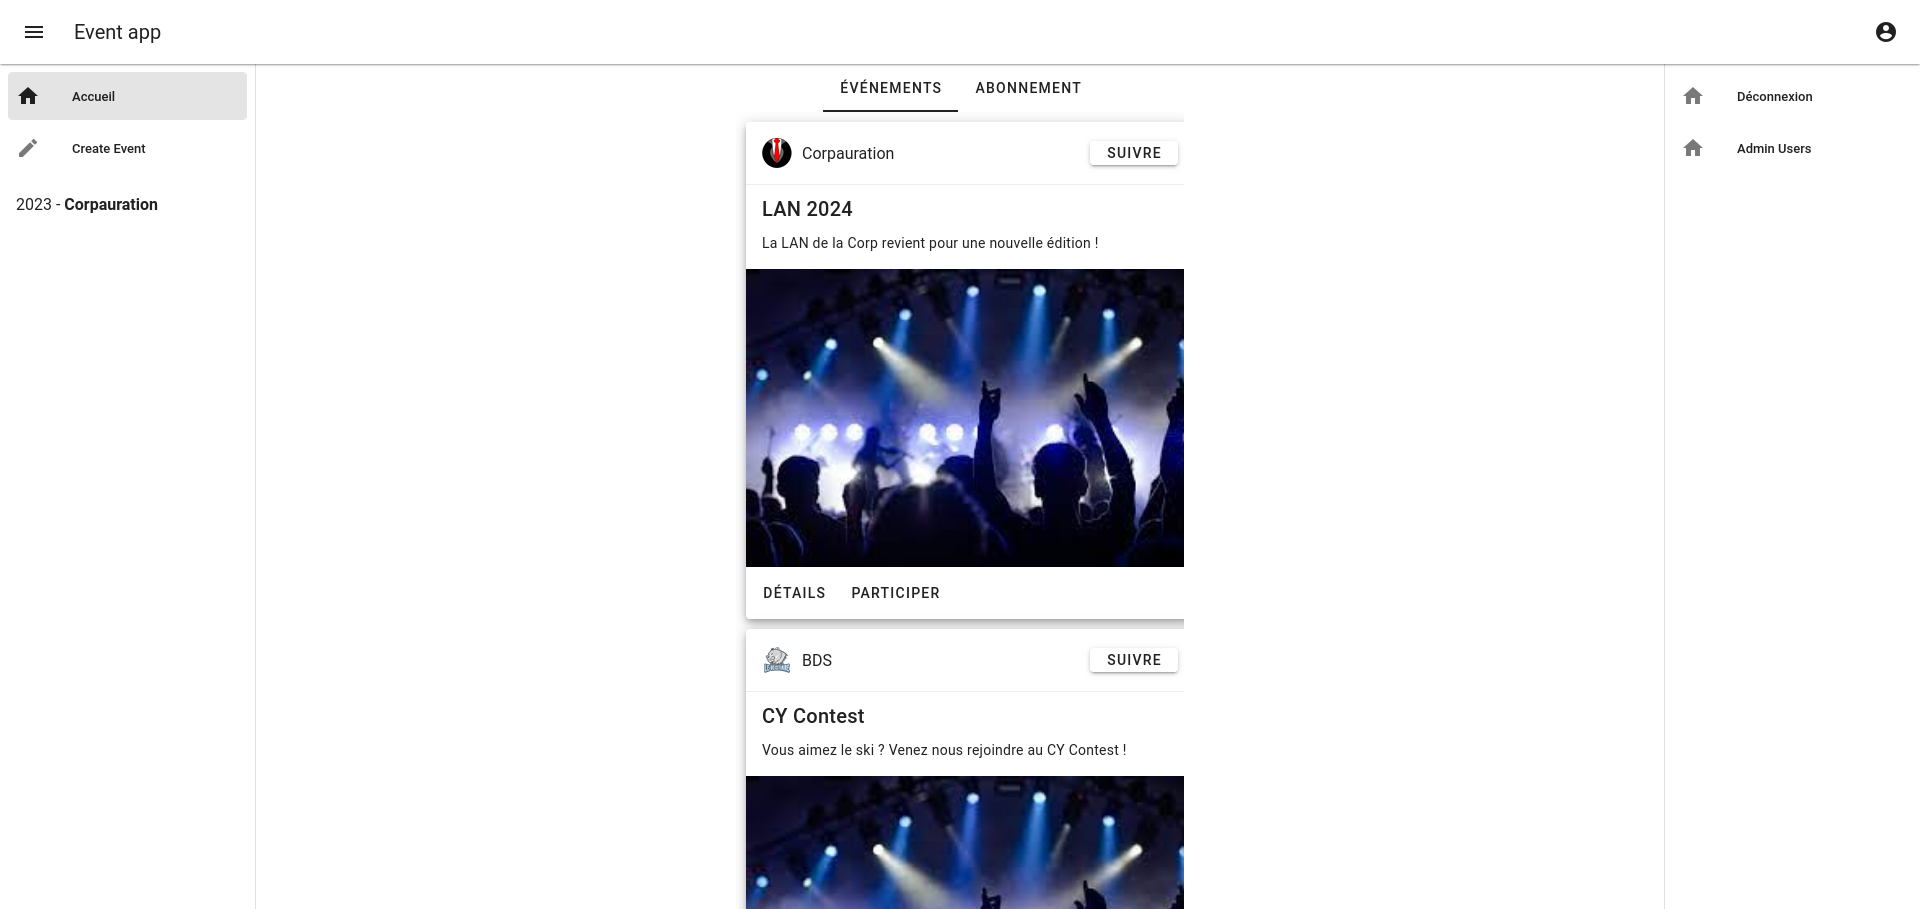
\includegraphics[width=0.95\textwidth]{assets/homepage.png}
	\caption{Page d'accueil}
	\label{fig:homepage}
\end{figure}


\begin{figure}[!h]
	\centering
	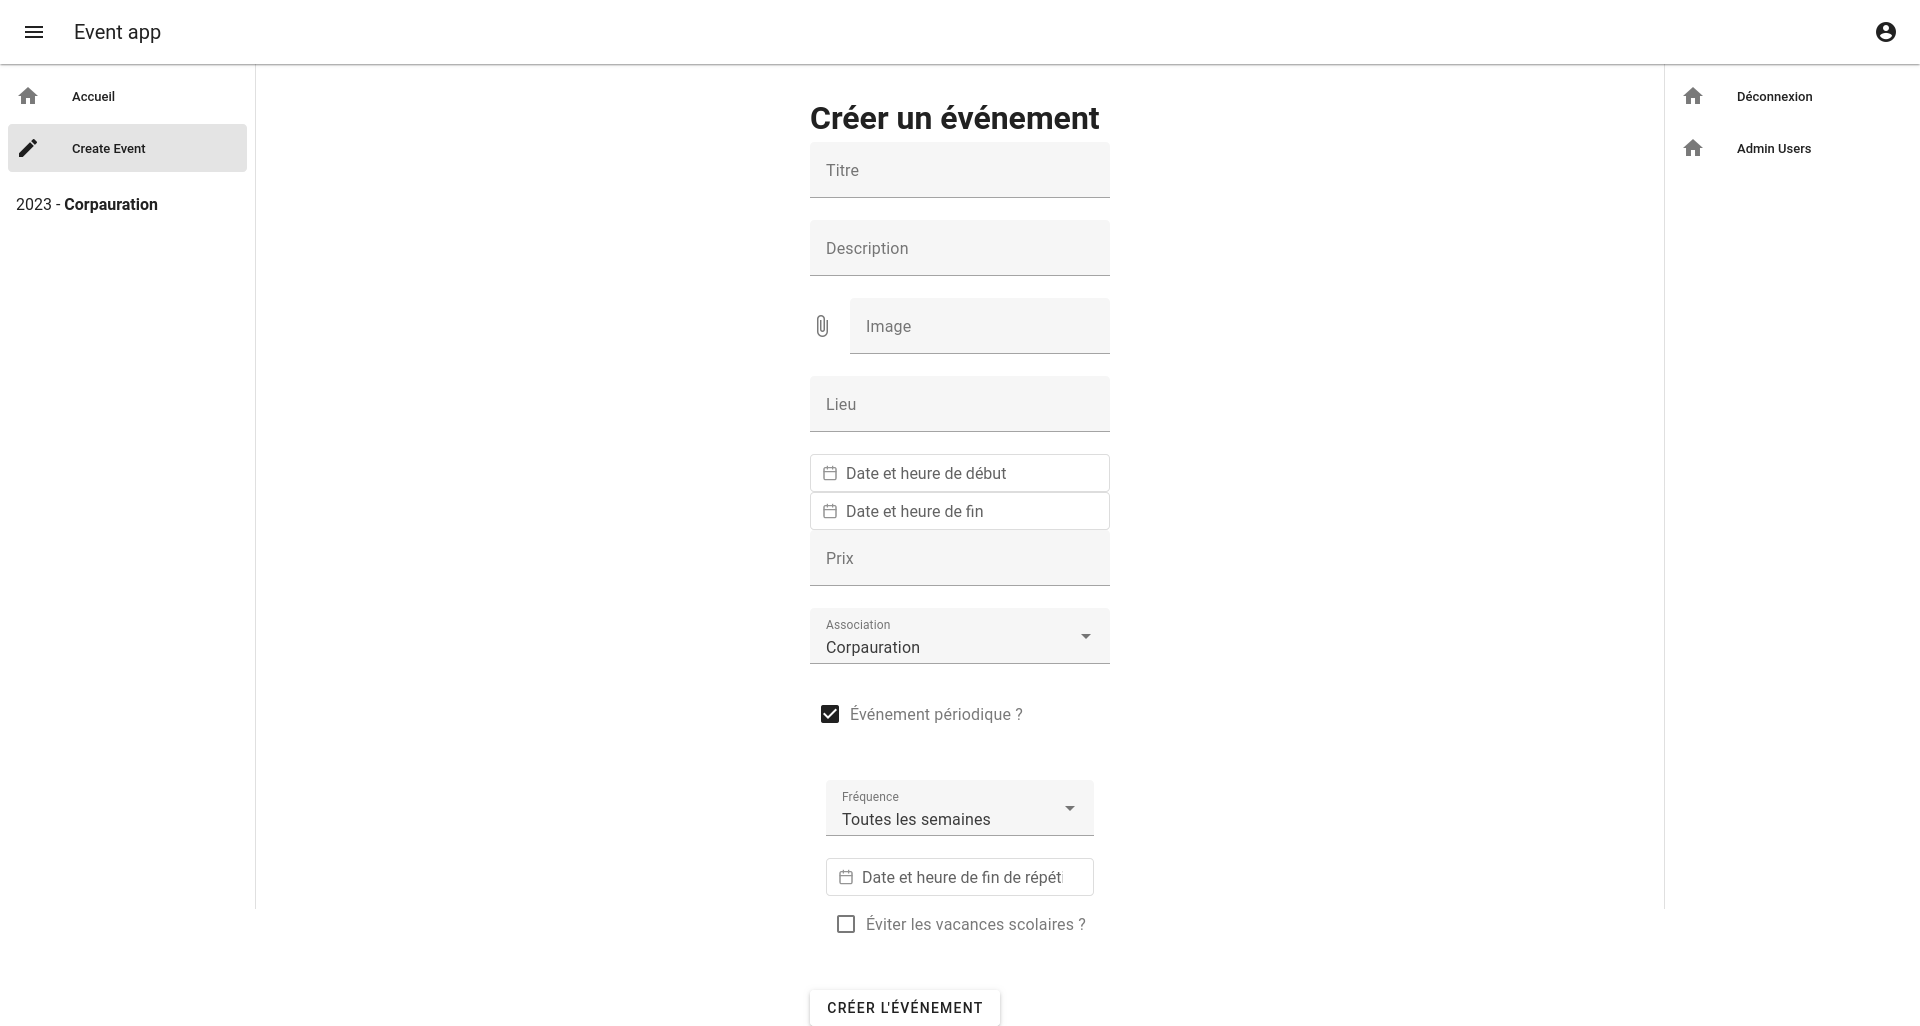
\includegraphics[width=0.95\textwidth]{assets/createevent.png}
	\caption{Page de création d'événements}
	\label{fig:createevent}
\end{figure}

% Il abordera les problèmes rencontrés, ainsi que la manière dont ils ont été gérés. Il devra expliquer les solutions adoptées et celles qu’il aurait fallu adopter.

\subsection{Analyse}

Dans cette section, nous explorerons en détail le développement de l'application web et de l'API, ainsi que les difficultés rencontrées tout au long de cette période de stage.

\subsubsection{La communication}

La communication joue un rôle crucial dans le développement de tout projet, mais elle peut présenter des défis particuliers, comme nous l'avons constaté dans le cadre de ce projet.

\medskip

Mon stage s'est déroulé au sein d'une association étudiante. Les membres de cette association n'étaient pas disponibles en permanence, car ils avaient leurs propres responsabilités, stages et engagements. Cette contrainte a parfois limité les créneaux pour les échanges en temps réel.

Pour résoudre ce problème, nous avons mis en place deux solutions. Tout d'abord, nous avons créé un salon sur Discord, une plateforme de messagerie, regroupant le second stagiaire, mon maître de stage, les membres du bureau de l'association et moi-même. Cette solution nous a permis de discuter des différents aspects du stage, de partager nos problématiques et d'organiser des réunions pour faire le point sur l'avancement des projets. Ensuite, nous avons tiré parti des fonctionnalités d'issues et de versioning offertes par Git et GitHub. Le versioning assure un contrôle de l'évolution du logiciel en créant des sauvegardes à chaque étape du développement. Le système d'issues permet de noter des idées ou des problèmes liés au logiciel. Cela permet à tous les participants du projet de suivre les nouvelles idées et les problèmes, de s'attribuer les tâches et de collaborer efficacement, même sans communication en temps réel.

\medskip

La distance géographique représente un autre obstacle à la communication. Ne pas se croiser physiquement dans un bureau et ne pas pouvoir obtenir une réponse immédiate en cas de problème peuvent poser des défis. Toutefois, cette situation présente des avantages : travailler sans interruption, gérer son propre emploi du temps de manière flexible et développer des compétences d'auto-apprentissage.

\medskip

Nous avons constaté que bien que la communication puisse être plus complexe dans un environnement associatif en télétravail, les technologies modernes et les méthodes de collaboration adaptées peuvent surmonter ces défis et exploiter les avantages offerts par le travail à distance.

\begin{figure}
	\centering
	\begin{subfigure}{.45\textwidth}
		\centering
		
\includegraphics[width=0.40\textwidth]{assets/discord.jpg}
		\subcaption{Discord}
		\label{fig:discord}
	\end{subfigure}
	\begin{subfigure}{.45\textwidth}
		\centering
		
\includegraphics[width=0.40\textwidth]{assets/github.png}
		\subcaption{GitHub}
		\label{fig:github}
	\end{subfigure}
	\caption{Technologies utilisées pour la communication et le versioning}
\end{figure}


\subsubsection{L'apprentissage de nouvelles technologies}

Ce projet m'a confronté à l'apprentissage de sept nouvelles technologies distinctes, dont aucune ne m'était familière. Cette opportunité d'apprentissage m'a permis de développer de nouvelles compétences tout au long du processus, bien que j'aie commencé à me familiariser avec certaines de ces technologies avant le début du stage.

L'apprentissage de la majorité de ces technologies s'est avéré être un processus relativement fluide. Certaines présentaient des similarités avec des technologies que j'avais déjà utilisées (comme Vue et React qui reposent sur un système de composants, ou Kotlin qui est une amélioration de Java). De plus, certaines de ces technologies étaient bien documentées.

Ma démarche pour assimiler ces nouvelles technologies a consisté en plusieurs étapes. J'ai commencé par visionner des vidéos de présentation des concepts fondamentaux. Ensuite, j'ai entrepris de créer une petite application de liste de tâches (To-Do List) en suivant des tutoriels. Cette approche m'a permis de prendre en main les technologies en pratique tout en bénéficiant d'une orientation structurée. Enfin, j'ai approfondi mes connaissances en consultant les documentations spécifiques à chaque technologie.

Cette démarche d'apprentissage m'a permis d'acquérir rapidement les compétences nécessaires pour contribuer de manière efficace au projet et pour surmonter les défis liés à l'utilisation de nouvelles technologies.

\subsubsection{Le manque de documentation}

Un défi majeur que j'ai rencontré au cours du projet était le manque substantiel de documentation et de tutoriels, en particulier pour Quarkus et Hibernate. En effet, Quarkus est un framework relativement récent développé par RedHat. Bien qu'il ait gagné en popularité auprès de nombreux développeurs, son utilisation reste moins répandue par rapport à d'autres langages et frameworks. Par conséquent, contrairement à d'autres environnements où l'on peut généralement trouver des solutions à divers problèmes, ce n'était pas toujours le cas avec Quarkus. Un défi similaire s'est présenté avec Hibernate, où j'ai été confronté à une erreur qui avait été découverte un mois auparavant mais qui n'avait pas encore été corrigée par les développeurs.

Pour surmonter ce défi, j'ai souvent dû adopter une approche de résolution de problèmes différente. Cela impliquait de rechercher des situations similaires et d'adapter les solutions existantes à mes besoins, ou d'examiner des dépôts open-source sur des plateformes comme GitHub pour comprendre comment d'autres développeurs avaient abordé des problèmes similaires.

Cet aspect du projet a exigé de la créativité, de la persévérance et une volonté de penser de manière novatrice pour contourner les obstacles liés au manque de documentation. Malgré les défis, cette expérience m'a permis d'améliorer mes compétences en résolution de problèmes et de développer une meilleure compréhension des technologies en question.

\subsubsection{L'authentification}

La mise en place d'un système d'authentification sécurisé représente un élément essentiel au sein d'une application web. Cependant, c'est souvent l'un des aspects les plus complexes à implémenter, car il implique de nombreuses contraintes en matière de sécurité. Comment garantir que seuls les utilisateurs autorisés peuvent accéder à certaines données ? Comment prévenir les tentatives d'usurpation d'identité ?

C'est pourquoi nous avons opté pour l'utilisation d'un serveur d'authentification dédié qui se chargera de gérer ces aspects pour nous. Toutefois, cette approche a initialement posé des défis pour moi, car je ne comprenais pas complètement le fonctionnement de ce serveur. Pour résoudre cette problématique, j'ai entrepris de rechercher un dépôt open-source sur GitHub où l'extension Keycloak était utilisée. En analysant le code de ce dépôt, en le croisant avec les informations fournies dans la documentation, j'ai réussi à comprendre et à mettre en place le serveur d'authentification avec succès.

Cette expérience m'a non seulement permis de surmonter les difficultés liées à la mise en place de l'authentification, mais elle m'a également offert une opportunité d'apprentissage approfondi et de développement de compétences en utilisant des ressources existantes et en les adaptant à mes besoins spécifiques.

\subsubsection{La réactivité de l'API}

L'aspect le plus exigeant de mon stage a été la mise en place de la réactivité au niveau de l'API. Développer une application réactive signifie créer une application capable de traiter simultanément plusieurs requêtes de manière asynchrone. Cette approche permet de réduire le temps d'attente moyen pour chaque utilisateur, évitant ainsi qu'une requête doive attendre la fin de toutes les autres pour être traitée. En d'autres termes, cela autorise un grand nombre d'utilisateurs à interagir avec l'application simultanément sans subir de ralentissements.

Cependant, cette réalisation s'est avérée particulièrement complexe. La création d'une application réactive exige une manière de penser et de programmer inhabituelle, car les étapes de traitement ne se déroulent pas nécessairement dans un ordre linéaire. Il est possible qu'une fonction s'exécute neuf fois sur dix, mais échoue lors de la dixième parce qu'une tâche nécessaire à une autre n'a pas encore été achevée.

Ce sont précisément ces problèmes qui ont demandé le plus de temps pour être résolus. Dans cette situation, seule la patience et l'expérience du vice-président m'ont permis de surmonter ces difficultés. Cette expérience m'a enseignée l'importance cruciale de la réactivité dans le développement d'applications modernes et m'a offert une occasion d'apprendre grâce à des conseils avisés la résolution de problèmes complexes en collaboration.

\subsubsection{Le développement de micro-fonctionnalités}

La méthodologie de développement basée sur la création de micro-fonctionnalités a été une approche qui m'a été très bénéfique, m'offrant non seulement de la flexibilité, mais également un gain de temps appréciable.

L'idée centrale de cette approche consiste à développer l'application en construisant des composants de petite taille mais fonctionnels. À partir d'un composant de base, nous greffons progressivement de nouvelles fonctionnalités, créant ainsi une chaîne d'ajouts successifs. Cette méthode présente plusieurs avantages : elle favorise la flexibilité en permettant des ajustements constants, elle offre une visibilité claire sur l'état d'avancement du projet et elle garantit la disponibilité d'une application fonctionnelle à tout moment.

En outre, cette approche nous a permis de mettre l'application en production dès que possible. Nous visons en effet à rendre l'application accessible dès le début de la rentrée scolaire. Cependant, compte tenu du nombre étendu de fonctionnalités que nous souhaitions inclure, achever une application totalement aboutie dès la rentrée aurait été irréaliste. La méthodologie de micro-fonctionnalités nous a offert la possibilité de lancer une application entièrement fonctionnelle dès le début, tout en ayant la flexibilité d'ajouter de nouvelles fonctionnalités par la suite, sans mettre en péril le fonctionnement des anciennes. Ainsi, l'application peut s'améliorer progressivement au fil du temps grâce à l'ajout de nouvelles fonctionnalités, sans risquer de compromettre la stabilité existante lors de chaque modification.

En résumé, le développement en micro-fonctionnalités a été une approche clé dans la réussite du projet, contribuant à sa souplesse, à son efficacité et à sa capacité à évoluer de manière progressive tout en garantissant la disponibilité d'une application fonctionnelle dès le lancement.